\setAuthor{Erkki Tempel}
\setRound{lahtine}
\setYear{2018}
\setNumber{G 1}
\setDifficulty{2}
\setTopic{Geomeetriline optika}

\prob{Kärbes}
Kärbes asub kumerläätse fokaaltasandil, läätse optilisest peateljest kaugusel $a = \SI{1}{m}$, ning hakkab lendama läätse kahekordse fookuskauguse suunas kiirusega $v = \SI{0,5}{m/s}$. Läätse fookuskaugus on $f = \SI{1}{m}$. Millise kiirusega $u$ liigub kärbse kujutis sel hetkel, kui kärbse ja tema kujutise vaheline kaugus on minimaalne?
\begin{center}
	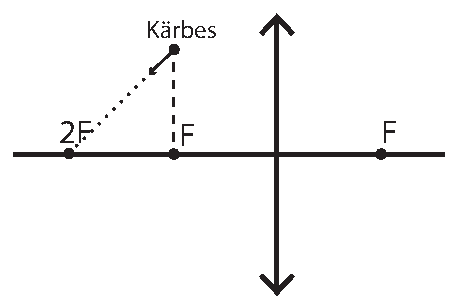
\includegraphics[width = 0.5\linewidth]{2018-lahg-01-yl.pdf}
\end{center}\hint
Kärbse ja tema kujutise vaheline kaugus on minimaalne siis, kui kärbes optilist peatelge läbib.\solu
Kärbse ja tema kujutise vaheline kaugus on minimaalne siis, kui kärbes läbib optilist peatelge. Kärbes ja tema kujutis on sel hetkel läätsest kahekordse fookuskauguse kaugusel. Tõepoolest, kärbse ja tema kujutise vahekaugus piki optilist peatelge on minimaalne siis, kui see asub $2f$ kaugusel läätsest (see on tuletatav läätse valemi kaudu) ning lisaks on sellel hetkel kärbse ja tema kujutise nihe piki läätse pinda minimaalne. Kuna nii kärbes kui ka tema kujutis on läätsest sama kaugel, on kujutise suurendus $1$, mistõttu kujutise liikumiskiirus on sama, mis kärbse liikumiskiirus, ehk $u = v = \SI{0,5}{m/s}$.\probend